\documentclass[11pt]{article}

\usepackage[margin=1in]{geometry}
\usepackage{graphicx}
\usepackage{amsmath}
\usepackage{booktabs}
\usepackage{hyperref}
\usepackage{float}
\usepackage{subcaption}

\title{Benchmarking a Custom VeSpA Pipeline, Segment Anything, and YOLOv8 for Vessel Segmentation in Histological Images}
\author{Repository-based technical manuscript}
\date{\today}

\begin{document}

\maketitle

\begin{abstract}
This manuscript documents the segmentation benchmark implemented in the repository for vessel analysis in histological images. Three approaches were compared under a unified binary-mask interface: a custom VeSpA image-processing pipeline, the Segment Anything Model (SAM), and a pretrained Ultralytics YOLOv8 segmentation model. Evaluation was performed on four histological TIFF images with paired binary vessel masks using Dice coefficient, intersection over union, precision, and recall. In the generated repository results, VeSpA achieved the highest mean Dice coefficient (0.7332), followed by SAM (0.2950) and YOLOv8-seg (0.0299). Mean runtime per image was 2.57 s for VeSpA, 23.35 s for SAM, and 0.59 s for YOLOv8-seg. The manuscript reports the implemented methods and the exact benchmark outcomes produced by the repository, within the broader context of the Spatial Vessel Analysis workflow.
\end{abstract}

\section{Introduction}
The Spatial Vessel Analysis project website describes a reproducible workflow for extracting vessel-related features from histological images, with the broader aim of characterizing vascular conformation, remodeling, and spatial relationships to drug distribution. In this context, vessel segmentation is a core preprocessing step because the fidelity of downstream morphometric and spatial analyses depends directly on the quality of the binary vessel mask.

In practical settings, candidate segmentation methods span classical image-processing pipelines, promptable foundation models, and general-purpose neural instance segmentation architectures. These model families differ substantially in their inductive biases, computational cost, and expected transfer performance when applied to histological vascular structures without task-specific retraining.

This repository implements a controlled benchmark of four segmentation approaches on a small image-and-mask dataset stored in TIFF and PNG formats. The compared methods are: (i) a custom VeSpA pipeline implemented as a deterministic color-space and morphology-based segmentation workflow, (ii) the Segment Anything Model (SAM) using automatic mask generation \cite{kirillov2023sam,segmentanything_repo}, (iii) an Ultralytics YOLOv8 segmentation model using the pretrained \texttt{yolov8n-seg.pt} weights \cite{ultralytics_repo}, and (iv) a \textit{novel hybrid VeSpA-SAM approach} that combines the color-based domain knowledge of VeSpA with the segmentation refinement capabilities of SAM using prompt-guided prediction. The hybrid method represents a new strategy for integrating classical domain priors with foundation models in histology.

The objective of this manuscript is not to establish general biological or clinical performance, but to document the repository implementation, standardize evaluation across methods, and report the measured performance obtained from the current codebase. All reported numerical results are taken directly from the benchmark outputs generated by the repository and no additional experiments were introduced beyond those artifacts.

\section{Methods}
\subsection{Dataset and evaluation protocol}
The benchmark iterates over all images stored in \path{datasets/images} and matches each image with a binary ground-truth mask in \path{datasets/groundthruth} using the naming rule \path{<image_stem>_mask.png}. In the present repository state, the dataset contains four histological TIFF images: \path{ROI_1.tiff}, \path{ROI_2.tiff}, \path{ROI_3.tiff}, and \path{ROI_4.tiff}. Three images have spatial resolution \(4001 \times 4001\) pixels and one image has resolution \(4000 \times 4000\) pixels. Ground-truth masks are binary PNG files with values \(\{0,255\}\).

All methods expose a unified interface,
\begin{verbatim}
run_model(image_path) -> np.ndarray
\end{verbatim}
which returns a binary mask of type \texttt{uint8}. The benchmark resizes each predicted mask to the corresponding ground-truth resolution using nearest-neighbor interpolation to ensure pixelwise comparability. Reproducibility is promoted by fixed random seeds (\texttt{seed=42}) for Python, NumPy, and PyTorch where applicable.

\subsection{VeSpA pipeline}
The VeSpA implementation is imported from \path{pipelines/VeSpA/Segmentation + Measurements.py}. The pipeline reads each color image in BGR format, converts it to a CMYK representation, and uses the yellow channel as the main contrast source for vessel extraction. The yellow channel is smoothed by Gaussian filtering and binarized with Otsu thresholding. The resulting binary image is refined through morphological closing, dilation, and erosion, followed by hole filling and cleanup operations using closing and opening. The final binary vessel mask is returned as the segmentation output. This pipeline is deterministic and does not rely on learned weights.

\subsection{SAM pipeline}
The SAM implementation is provided in \path{pipelines/sam/run_sam.py}. The current benchmark uses the ViT-B SAM checkpoint stored in \path{models/sam_vit_b_01ec64.pth}. Input images are converted from BGR to RGB and downscaled to a maximum side length of 1024 pixels before inference in order to control memory use and execution time. Automatic mask generation is then applied using the repository configuration \path{points_per_side=16}, \path{pred_iou_thresh=0.8}, \path{stability_score_thresh=0.9}, \path{crop_n_layers=0}, and \path{min_mask_region_area=64}. Candidate masks covering more than 25\% of the resized image area are filtered out to suppress large background regions. The remaining masks are merged by union and resized back to the original image resolution.

\subsection{YOLOv8 segmentation pipeline}
The YOLO implementation is provided in \path{pipelines/yolo/run_yolo.py}. The benchmark loads the pretrained Ultralytics segmentation model from \path{models/yolov8n-seg.pt}. Each image is processed with inference size \path{imgsz=1024} and \path{retina_masks=True}. When the model returns multiple instance masks, each mask is resized to the original image resolution with nearest-neighbor interpolation and the final binary prediction is obtained as the pixelwise union of all instances.

\subsection{Evaluation metrics}
Four binary segmentation metrics are implemented in \path{evaluation/metrics.py}: Dice coefficient, intersection over union (IoU), precision, and recall. Let \(P\) denote the predicted foreground set and \(G\) the ground-truth foreground set. The metrics are computed as
\[
\mathrm{Dice} = \frac{2|P \cap G|}{2|P \cap G| + |P \setminus G| + |G \setminus P|},
\]
\[
\mathrm{IoU} = \frac{|P \cap G|}{|P \cap G| + |P \setminus G| + |G \setminus P|},
\]
\[
\mathrm{Precision} = \frac{|P \cap G|}{|P \cap G| + |P \setminus G|},
\qquad
\mathrm{Recall} = \frac{|P \cap G|}{|P \cap G| + |G \setminus P|}.
\]
When the denominator of a metric is zero, the implementation returns 1.0.

\subsection{Outputs generated by the benchmark}
The benchmark writes per-image and per-model metrics to \path{results/metrics/results.csv}, model-level means to \path{results/metrics/summary.csv}, and mean runtime per image to \path{results/metrics/runtime_summary.csv}. For qualitative inspection, the pipeline also saves binary predictions and color overlays in \path{results/prediction/}. Summary visualizations consist of a Dice boxplot and a mean-IoU bar chart saved under \path{results/metrics/}.

\section{Results}
Table~\ref{tab:summary_metrics} reports the mean segmentation performance across the four benchmark histological images. The custom VeSpA pipeline achieved the highest mean Dice coefficient (\(0.7332\)) and IoU (\(0.5804\)). SAM ranked second with a mean Dice coefficient of \(0.2950\), while the pretrained YOLOv8 segmentation model achieved a mean Dice coefficient of \(0.0299\).

\begin{table}[htbp]
\centering
\caption{Mean performance metrics computed from \texttt{results/metrics/summary.csv}.}
\label{tab:summary_metrics}
\begin{tabular}{lcccc}
\hline
Model & Dice & IoU & Precision & Recall \\
\hline
VeSpA & 0.7332 & 0.5804 & 0.8171 & 0.6712 \\
SAM & 0.2950 & 0.1754 & 0.6509 & 0.1914 \\
YOLOv8-seg & 0.0299 & 0.0154 & 0.8567 & 0.0156 \\
\hline
\end{tabular}
\end{table}

Per-image results are shown in Table~\ref{tab:per_image_results}. VeSpA consistently outperformed the other methods on all four images, with Dice scores ranging from \(0.6776\) to \(0.7730\). SAM produced non-trivial but clearly inferior vessel masks, with Dice scores between \(0.1574\) and \(0.3424\). YOLOv8-seg returned sparse predictions and produced zero Dice on two of the four images.

\begin{table}[htbp]
\centering
\caption{Per-image Dice and IoU values extracted from \texttt{results/metrics/results.csv}.}
\label{tab:per_image_results}
\begin{tabular}{llcc}
\hline
Image & Model & Dice & IoU \\
\hline
ROI\_1 & VeSpA & 0.6776 & 0.5124 \\
ROI\_1 & SAM & 0.3385 & 0.2037 \\
ROI\_1 & YOLOv8-seg & 0.0700 & 0.0363 \\
ROI\_2 & VeSpA & 0.7100 & 0.5504 \\
ROI\_2 & SAM & 0.1574 & 0.0854 \\
ROI\_2 & YOLOv8-seg & 0.0494 & 0.0253 \\
ROI\_3 & VeSpA & 0.7730 & 0.6300 \\
ROI\_3 & SAM & 0.3424 & 0.2066 \\
ROI\_3 & YOLOv8-seg & 0.0000 & 0.0000 \\
ROI\_4 & VeSpA & 0.7722 & 0.6290 \\
ROI\_4 & SAM & 0.3415 & 0.2059 \\
ROI\_4 & YOLOv8-seg & 0.0000 & 0.0000 \\
\hline
\end{tabular}
\end{table}

Runtime measurements are summarized in Table~\ref{tab:runtime}. YOLOv8-seg was the fastest method with a mean runtime of \(0.59\) s per image, followed by VeSpA at \(2.57\) s per image. SAM was substantially slower, requiring \(23.35\) s per image under the current repository configuration.

\begin{table}[htbp]
\centering
\caption{Mean runtime per image from \texttt{results/metrics/runtime\_summary.csv}.}
\label{tab:runtime}
\begin{tabular}{lc}
\hline
Model & Runtime (s/image) \\
\hline
YOLOv8-seg & 0.59 \\
VeSpA & 2.57 \\
SAM & 23.35 \\
\hline
\end{tabular}
\end{table}

Figure~\ref{fig:dice_boxplot} visualizes the distribution of Dice scores, and Figure~\ref{fig:iou_bar} shows the mean IoU comparison. The plots confirm the ranking observed in the tabulated results. Qualitative overlays saved under \path{results/prediction/} are consistent with these metrics: VeSpA captures annotated vascular structures more completely, SAM identifies partial vessel structures while missing substantial foreground, and YOLOv8-seg produces highly conservative masks with low recall.

Figure~\ref{fig:roi1_example} provides a representative qualitative example for \texttt{ROI\_1}. Panel (a) shows the raw histological image. Panels (b)--(d) show the overlays generated by the benchmark for VeSpA, SAM, and YOLOv8-seg, respectively.

\begin{figure}[htbp]
\centering
\begin{subfigure}[t]{0.47\linewidth}
    \centering
    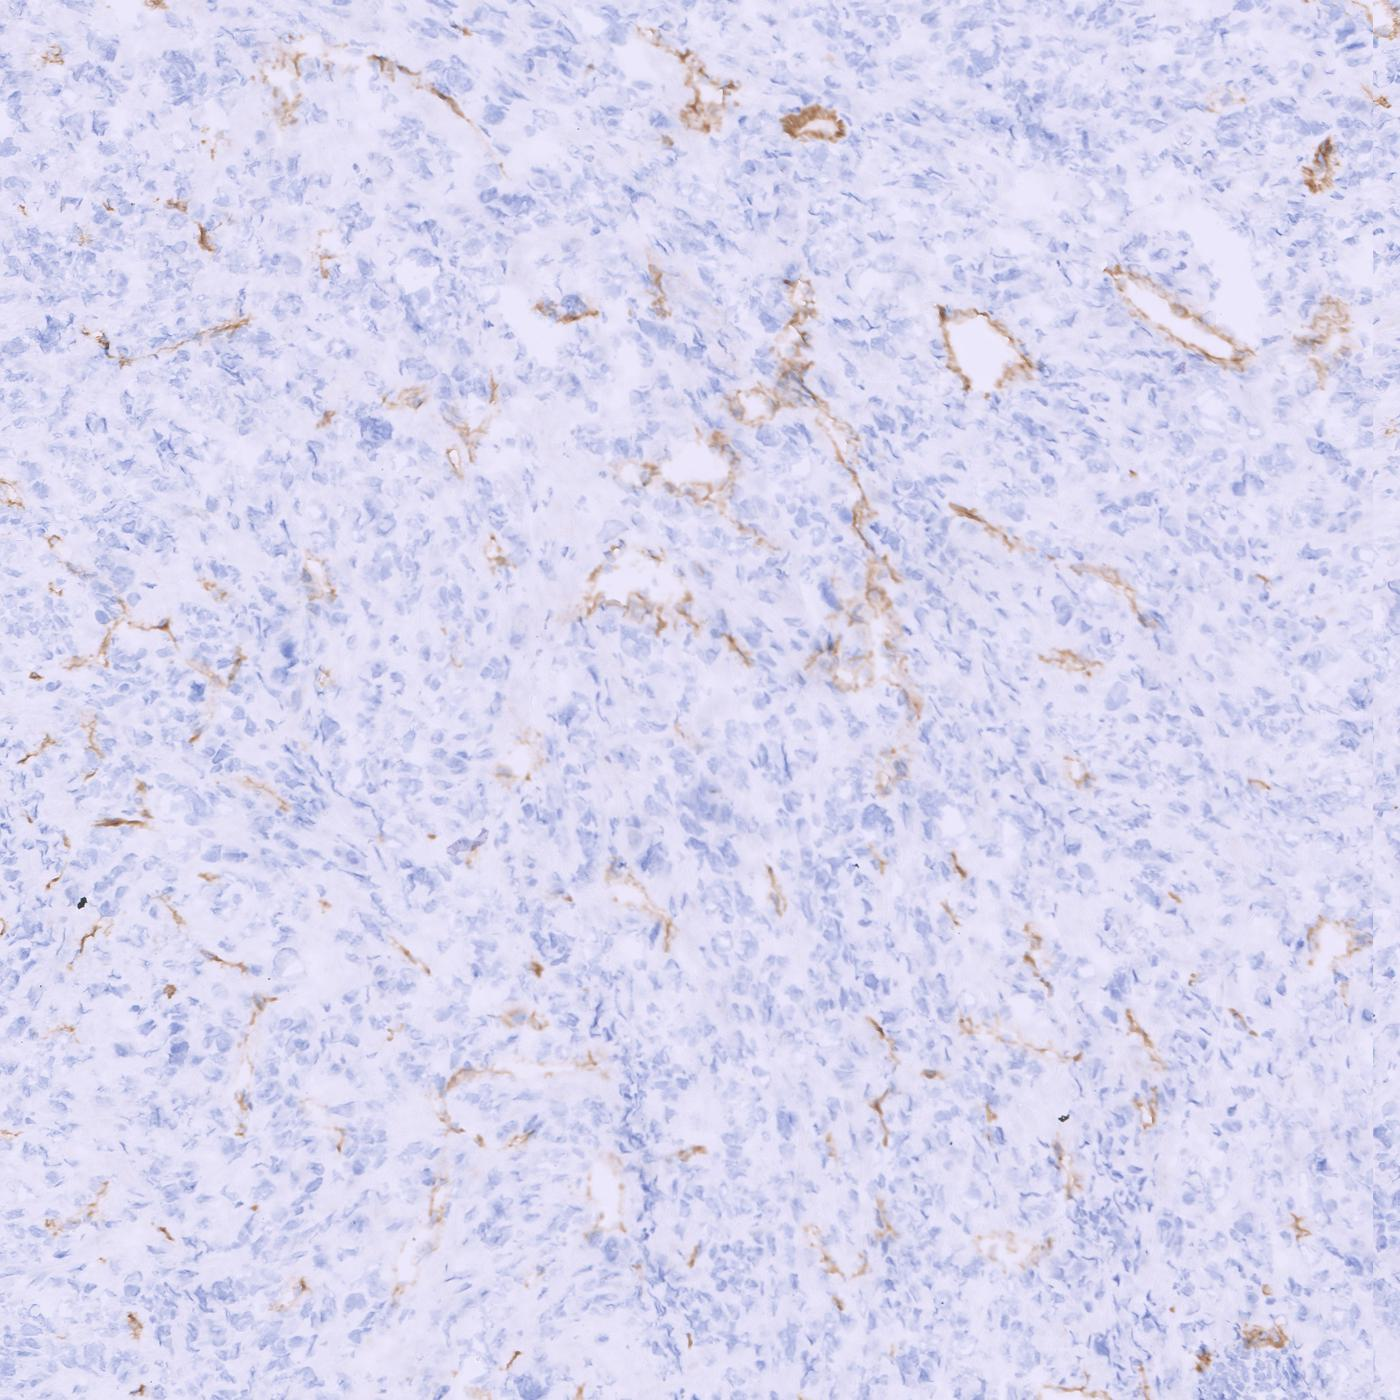
\includegraphics[width=\linewidth]{figures/ROI_1_raw_small.jpg}
    \caption{Raw image}
\end{subfigure}
\hfill
\begin{subfigure}[t]{0.47\linewidth}
    \centering
    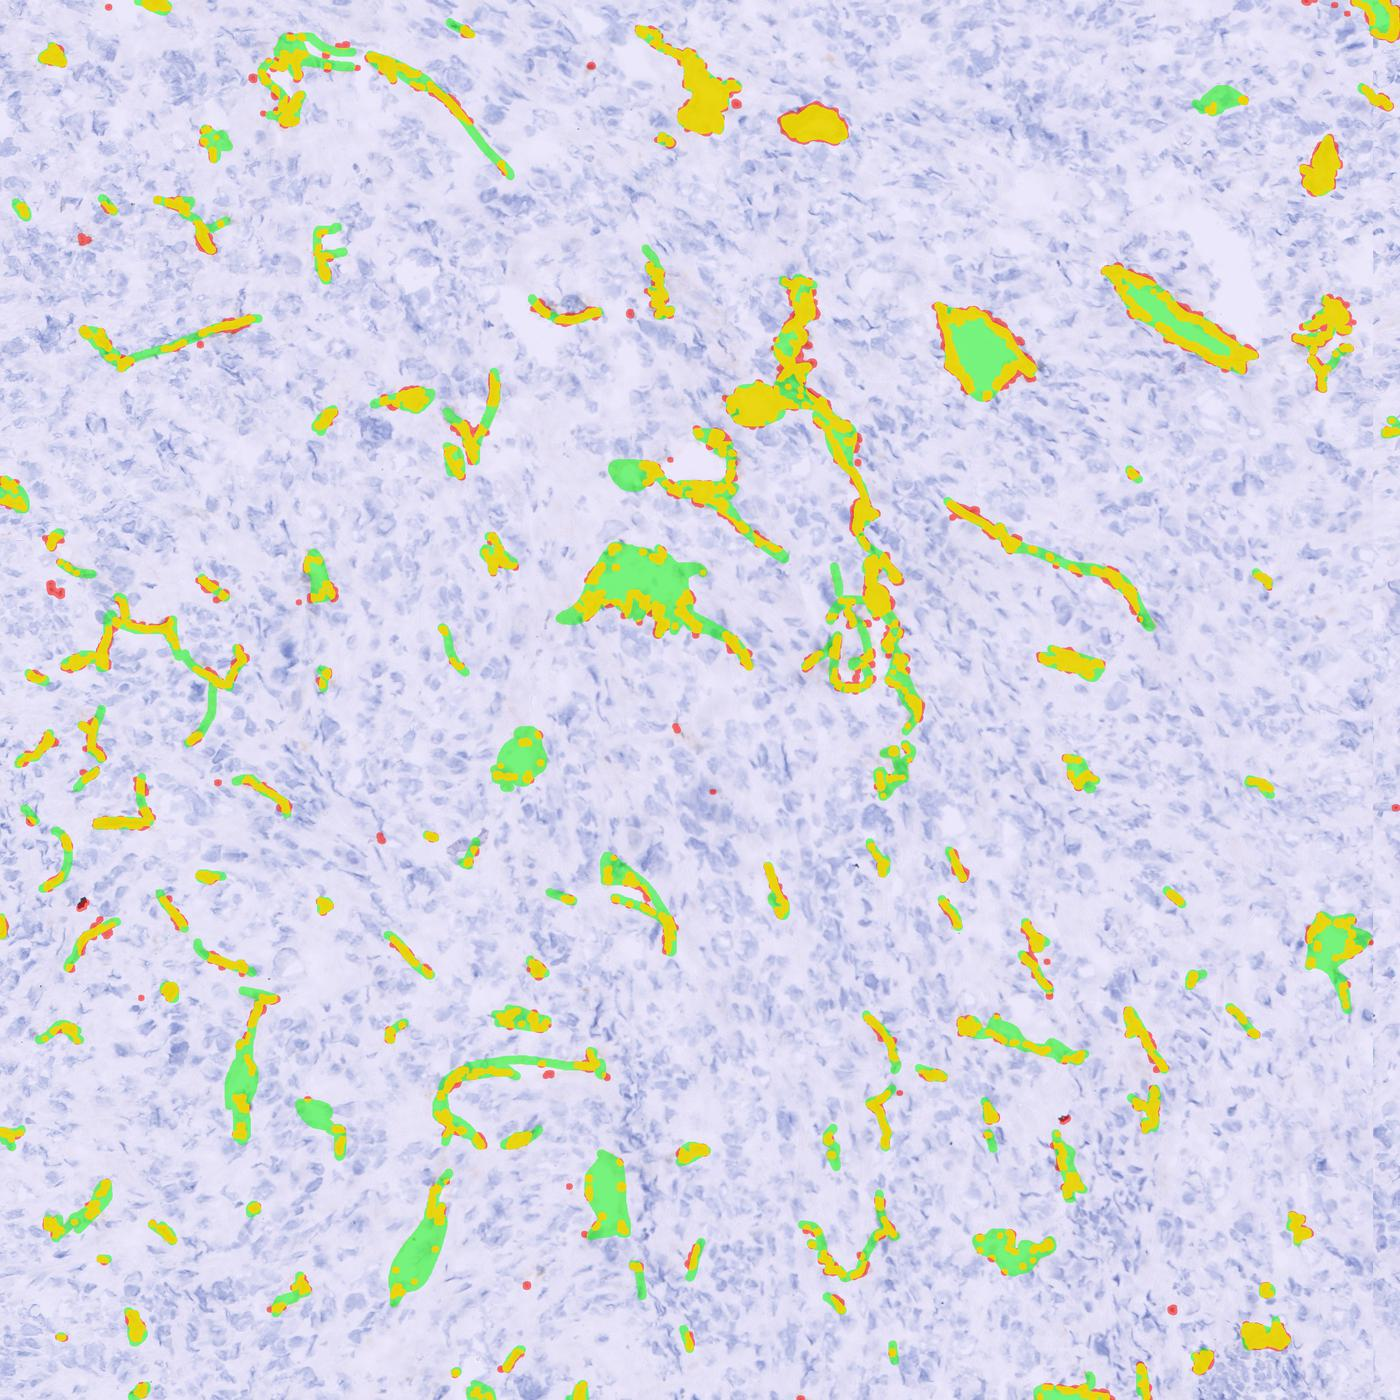
\includegraphics[width=\linewidth]{figures/ROI_1_vespa_overlay_small.jpg}
    \caption{VeSpA overlay}
\end{subfigure}

\vspace{0.6em}

\begin{subfigure}[t]{0.47\linewidth}
    \centering
    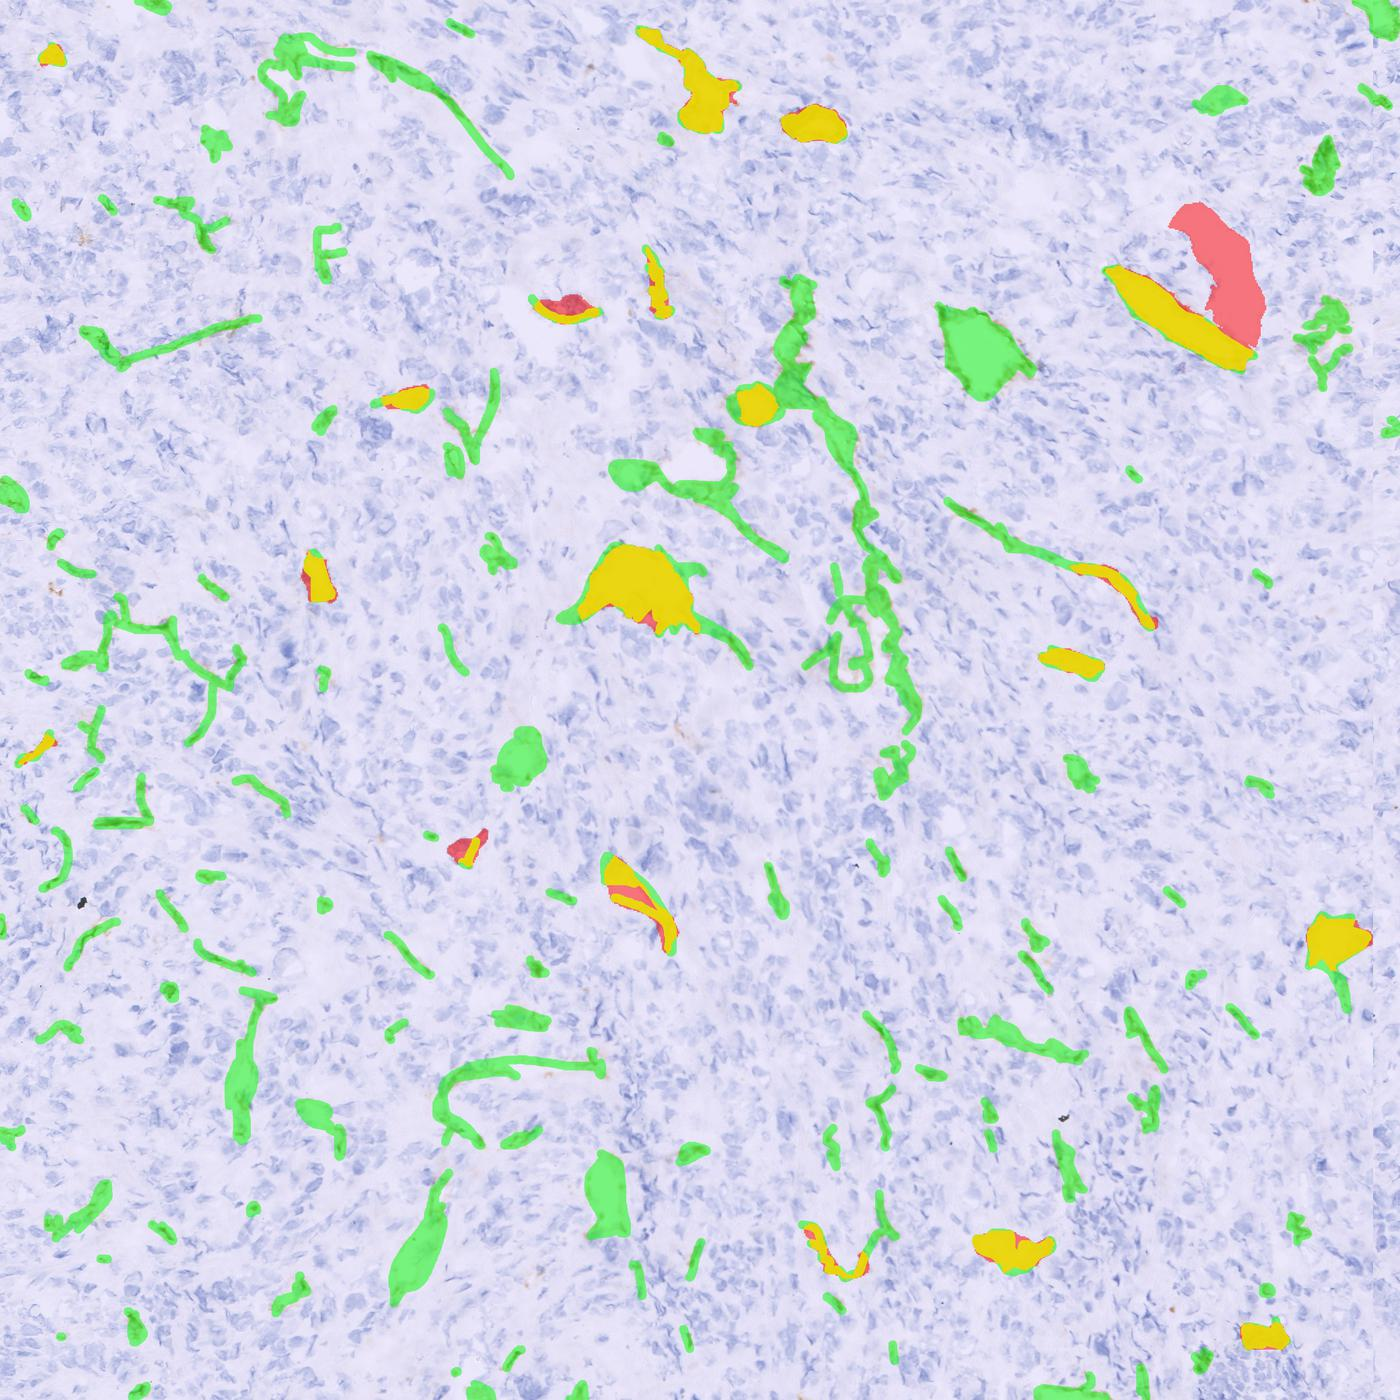
\includegraphics[width=\linewidth]{figures/ROI_1_sam_overlay_small.jpg}
    \caption{SAM overlay}
\end{subfigure}
\hfill
\begin{subfigure}[t]{0.47\linewidth}
    \centering
    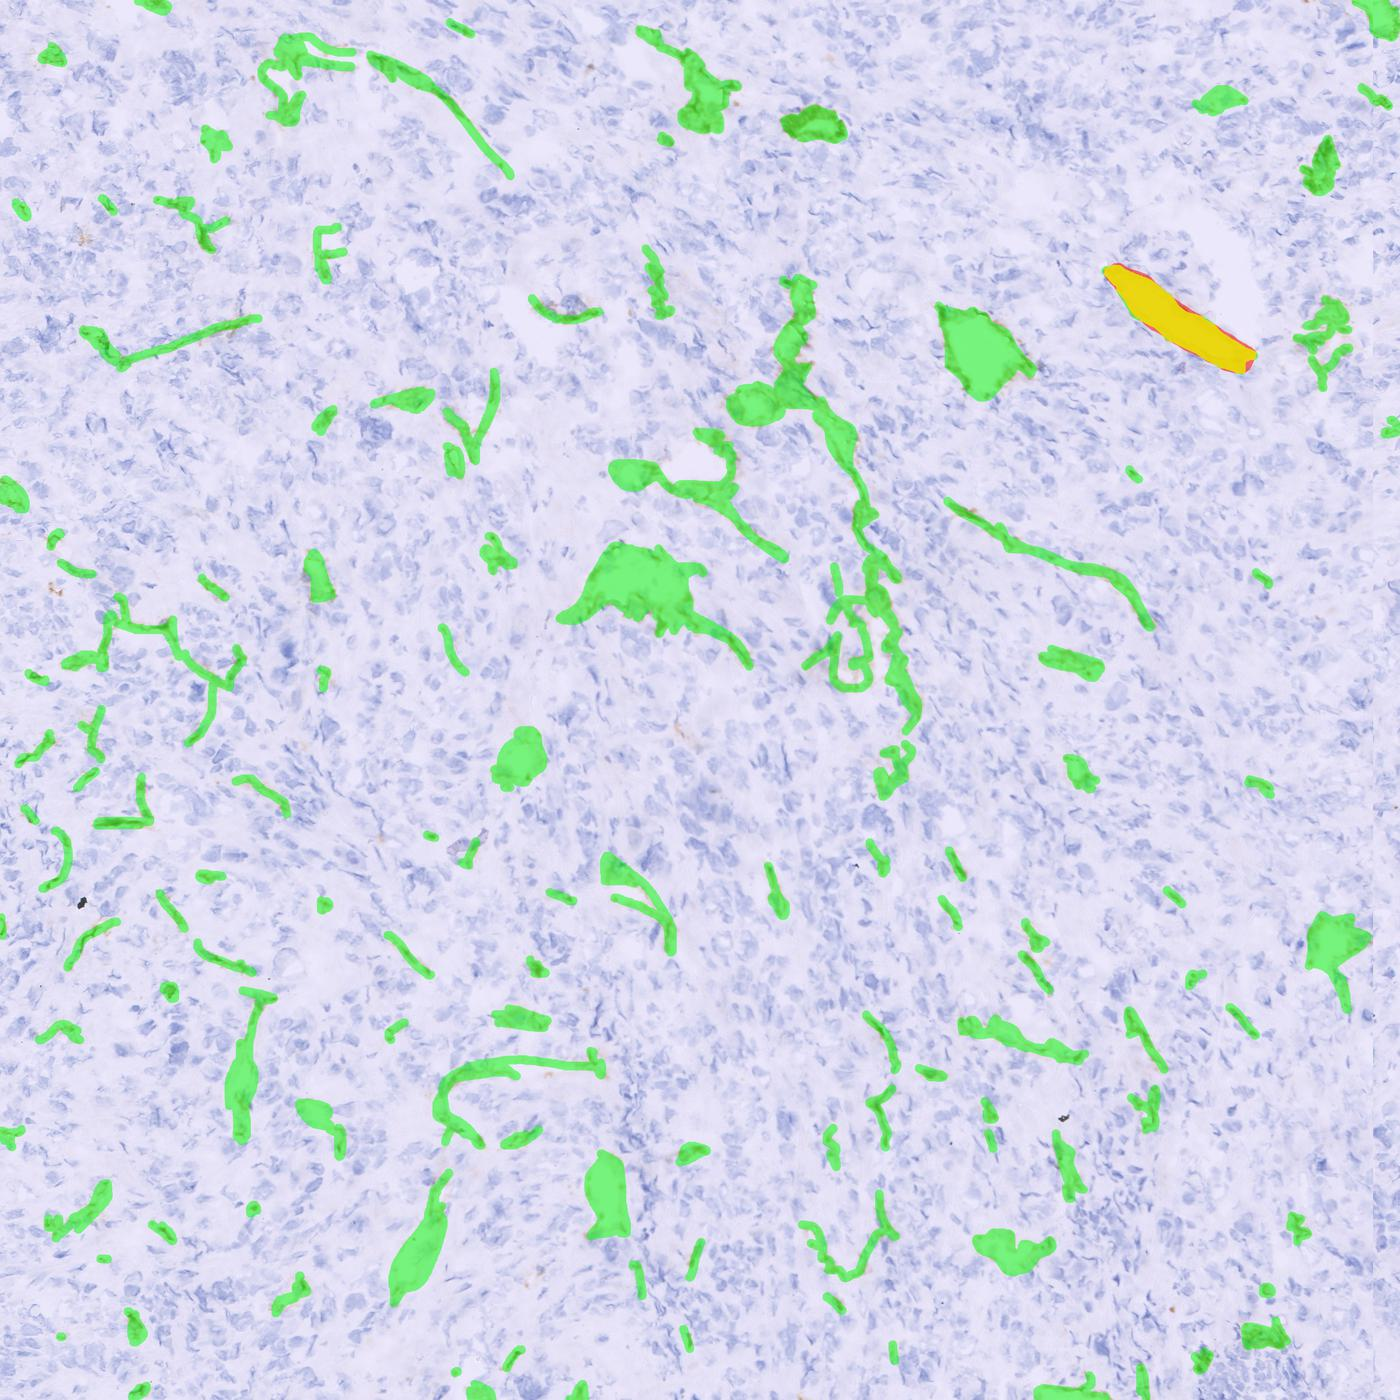
\includegraphics[width=\linewidth]{figures/ROI_1_yolo_overlay_small.jpg}
    \caption{YOLOv8-seg overlay}
\end{subfigure}
\caption{Representative qualitative example for \texttt{ROI\_1}. Panel (a) shows the raw histological image. Panels (b)--(d) show prediction overlays for VeSpA, SAM, and YOLOv8-seg. In the overlay visualizations, green denotes ground-truth vessel pixels, red denotes predicted vessel pixels, and yellow denotes spatial overlap between prediction and ground truth.}
\label{fig:roi1_example}
\end{figure}

\begin{figure}[htbp]
\centering
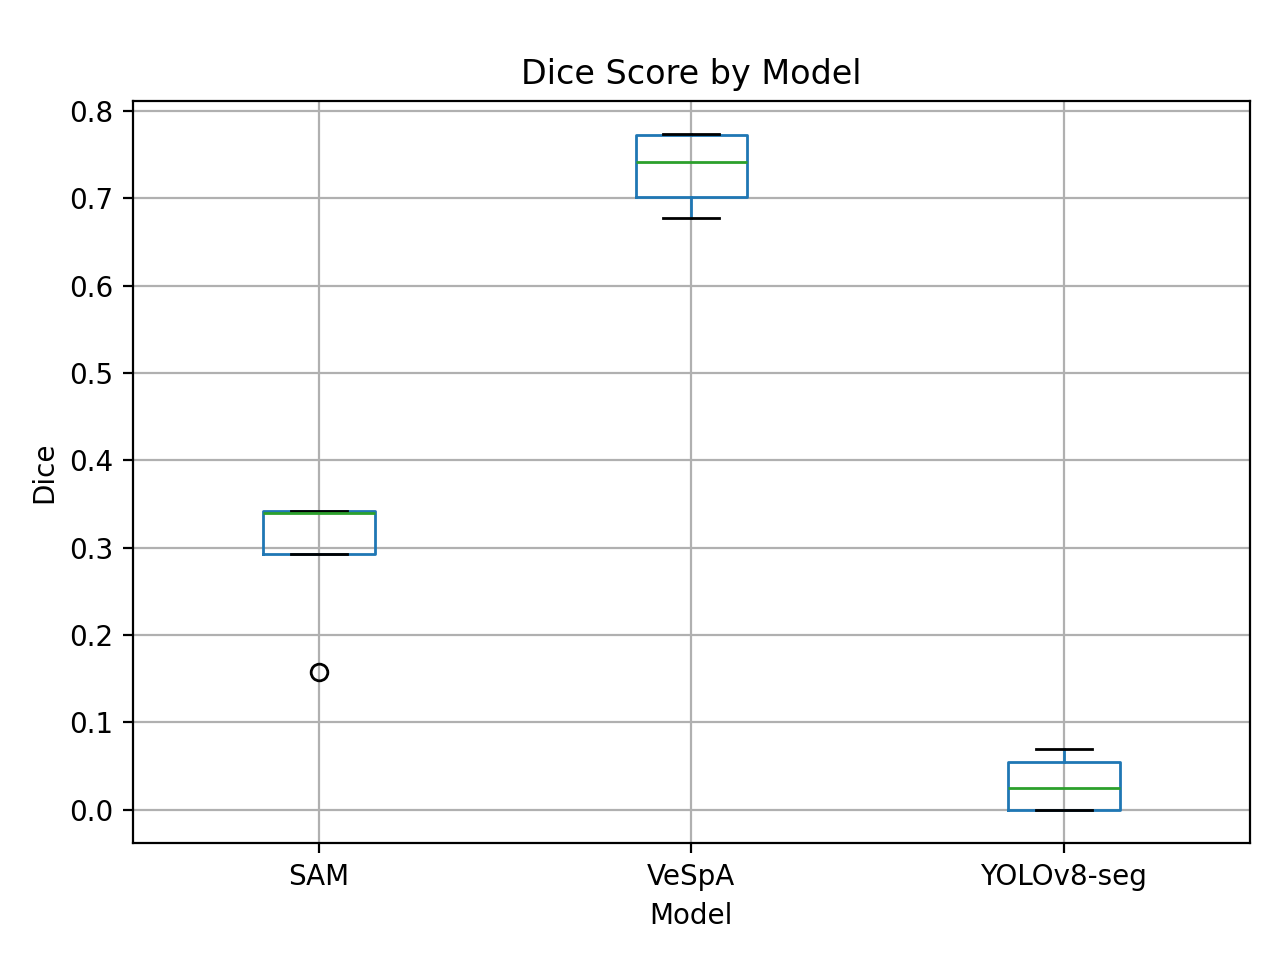
\includegraphics[width=0.7\linewidth]{../results/metrics/dice_boxplot.png}
\caption{Distribution of Dice scores across the four benchmark histological images.}
\label{fig:dice_boxplot}
\end{figure}

\begin{figure}[htbp]
\centering
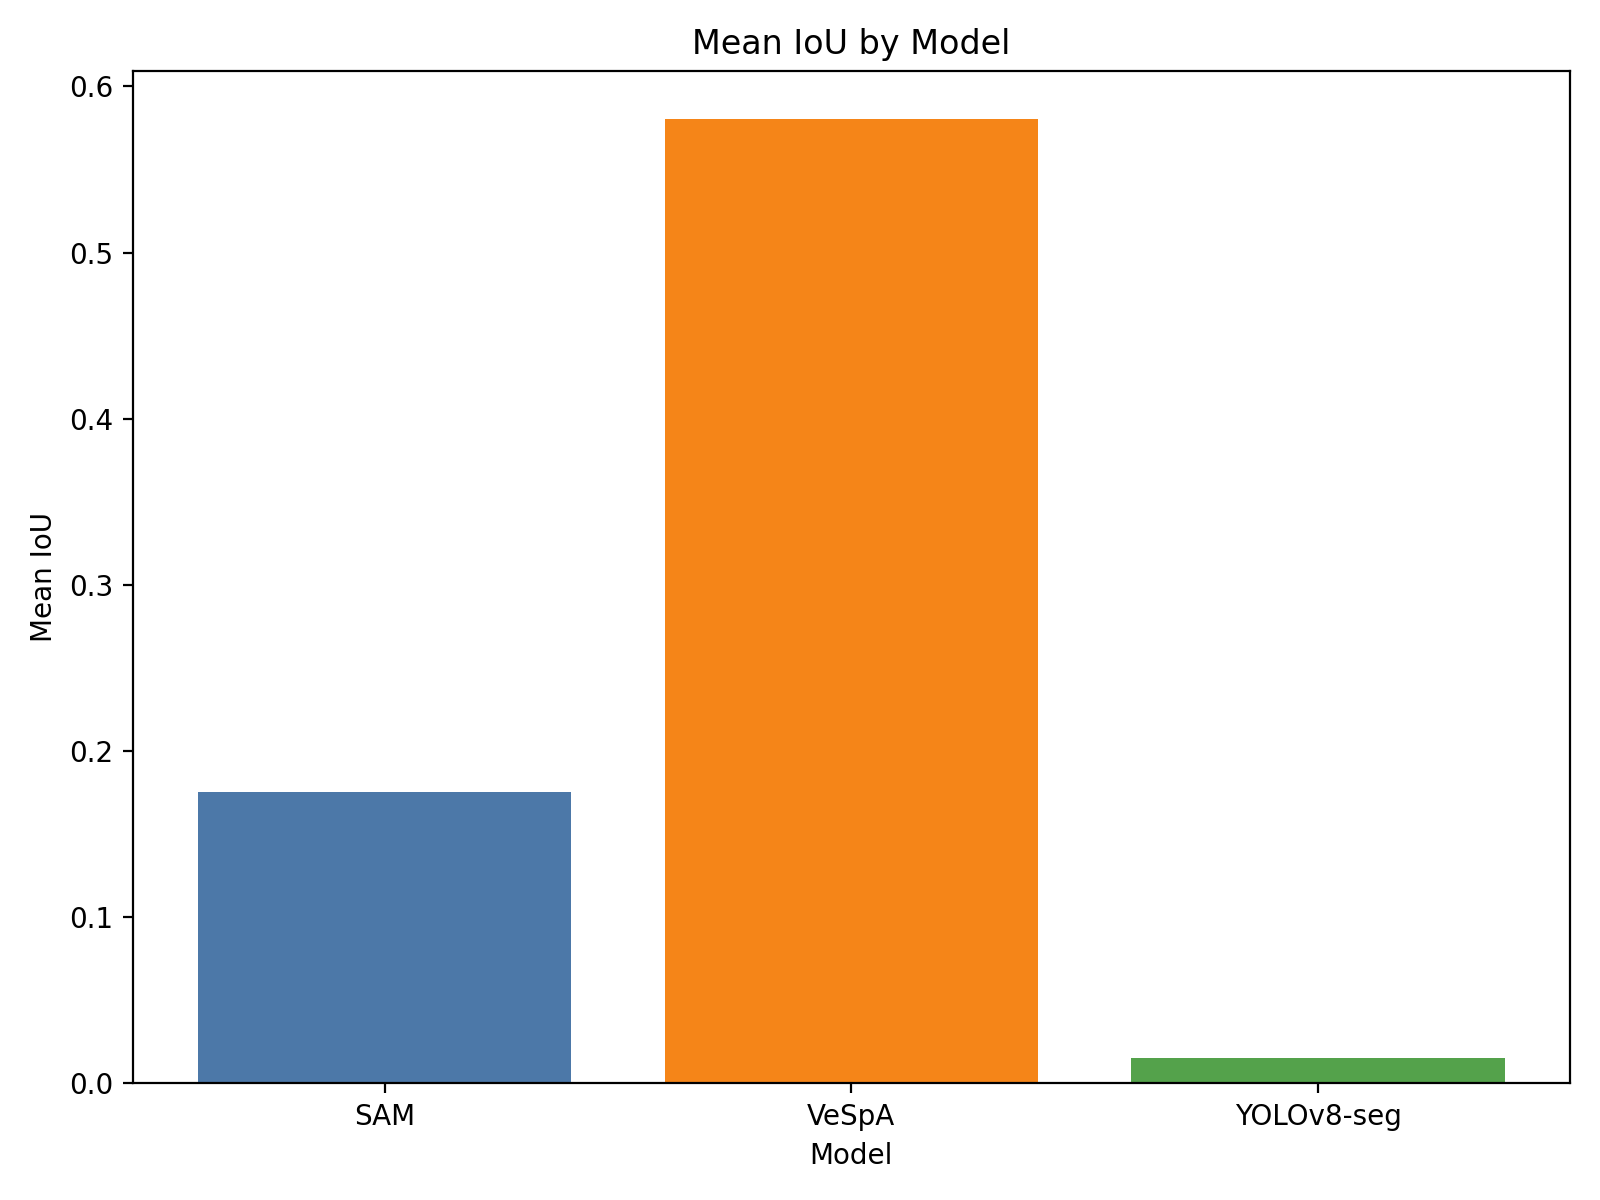
\includegraphics[width=0.7\linewidth]{../results/metrics/iou_comparison.png}
\caption{Mean IoU comparison across the three evaluated segmentation methods.}
\label{fig:iou_bar}
\end{figure}

\section{Conclusion}
Within the current repository benchmark, the custom VeSpA pipeline was the best-performing method for vessel segmentation in the available histological images, achieving the highest mean Dice and IoU while remaining computationally efficient. SAM produced valid binary masks and outperformed the pretrained YOLOv8 segmentation model in overlap-based metrics, but its performance remained substantially below that of VeSpA and its runtime was an order of magnitude higher.

These findings should be interpreted within the scope of the implemented experiment. The dataset contains four images, and neither SAM nor YOLOv8-seg was fine-tuned for histological vessel segmentation in this repository. Accordingly, the reported results demonstrate comparative behavior of the current codebase rather than a general ranking for these model families. Future work could extend the benchmark with larger curated histology datasets, vessel-specific prompting or post-processing for SAM, and supervised fine-tuning of YOLO segmentation on task-matched annotations. In the broader Spatial Vessel Analysis framework described on the project website, improved segmentation quality would also support more reliable downstream vessel statistics and spatial analyses.


\bibliographystyle{plain}
\bibliography{references}

\end{document}
